\section{Results}

\subsection{Virtual constraints controller}

When optimizing on the objective function~\ref{eq::virtual_constraints_objective_fun} with $w_1 = w_2 = 0.5$, and $\dot{x} = \SI{0.7}{\meter\per\second}$, the following set of optimized parameters were computed:

\begin{align*}
	\mathbf{q}_0 &= \begin{bmatrix}
		0.3239 \\ -0.3496 \\ \num{3.746e-4}
	\end{bmatrix} \\
	\mathbf{\dot{q}}_0 &= \begin{bmatrix}
		\num{2.894e-04} \\ \num{1.720e-04} \\ 8.583
	\end{bmatrix} \\
	k_{p1} &= 452.6 \\
	k_{p2} &= 102.1 \\
	k_{d1} &= 95.15 \\
	k_{d2} &= 4.619 \\
	\alpha &= 0.1911
\end{align*}

\begin{figure}[H]
	\begin{subfigure}[h]{0.495\textwidth}
		\begin{center}
			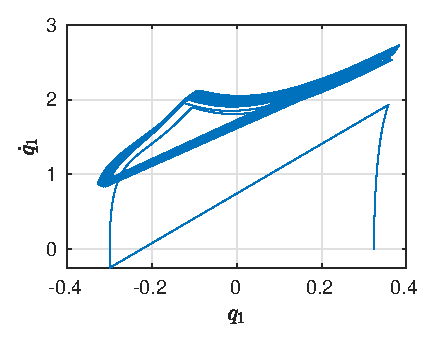
\includegraphics[width=\textwidth]{a04_state_space_q1_optimized}
			\caption{$q_1$ state-space plot}
%			\label{fig::img1}
		\end{center}
	\end{subfigure}
	\begin{subfigure}[h]{0.495\textwidth}
		\begin{center}
			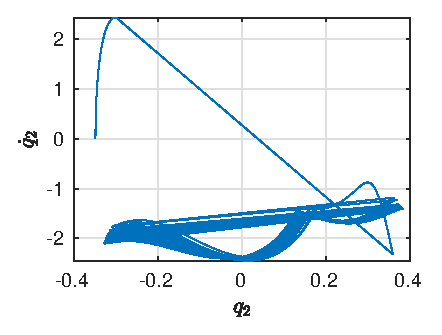
\includegraphics[width=\textwidth]{a04_state_space_q2_optimized}
			\caption{$q_1$ state-space plot}
%			\label{fig::img2}
		\end{center}
	\end{subfigure}

	\begin{subfigure}[h]{0.495\textwidth}
		\begin{center}
			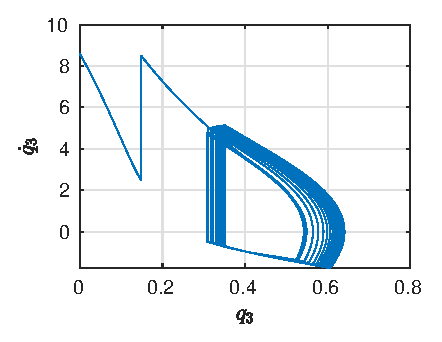
\includegraphics[width=\textwidth]{a04_state_space_q3_optimized}
			\caption{$q_1$ state-space plot}
%			\label{fig::img3}
		\end{center}
	\end{subfigure}
	\caption{State-space plot for the three generalized coordinates.}
%	\label{img::global_label}
\end{figure}

\begin{figure}[H]
	\begin{subfigure}[h]{0.495\textwidth}
		\begin{center}
			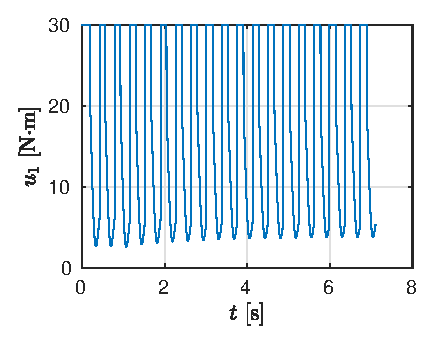
\includegraphics[width=\textwidth]{a04_control_torques_u1_optimized}
			\caption{first actuator}
		\end{center}
	\end{subfigure}
	\begin{subfigure}[h]{0.495\textwidth}
		\begin{center}
			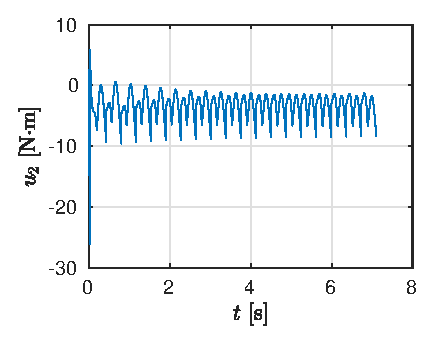
\includegraphics[width=\textwidth]{a04_control_torques_u2_optimized}
			\caption{second actuator}
		\end{center}
	\end{subfigure}
	\caption{Command angles in function of time for both actuators.}
\end{figure}

\begin{figure}[H]
	\begin{subfigure}[h]{0.8\textwidth}
		\begin{center}
			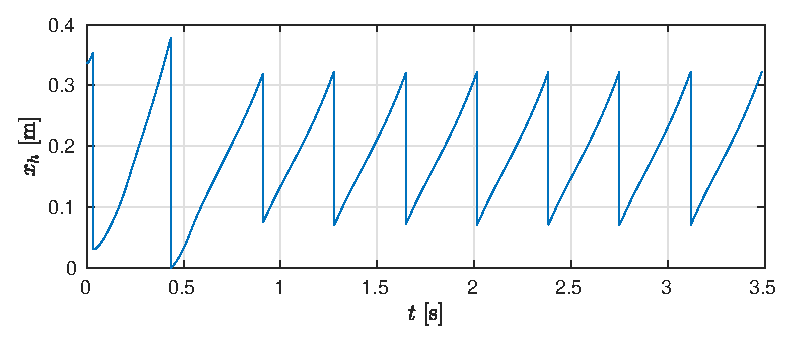
\includegraphics[width=\textwidth]{a04_x_h}
			\caption{horizontal position of the hip}
		\end{center}
	\end{subfigure}
	\begin{subfigure}[h]{0.8\textwidth}
		\begin{center}
			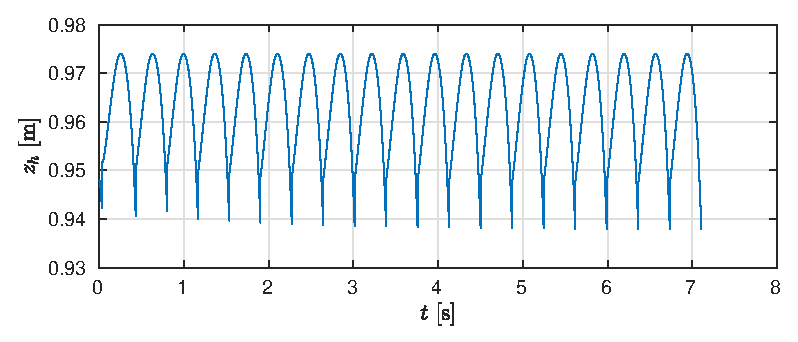
\includegraphics[width=\textwidth]{a04_z_h}
			\caption{vertical position of the hip}
		\end{center}
	\end{subfigure}
	\caption{Position of the hip as a function of time.}
\end{figure}

\begin{figure}[H]
	\begin{subfigure}[h]{0.495\textwidth}
		\begin{center}
			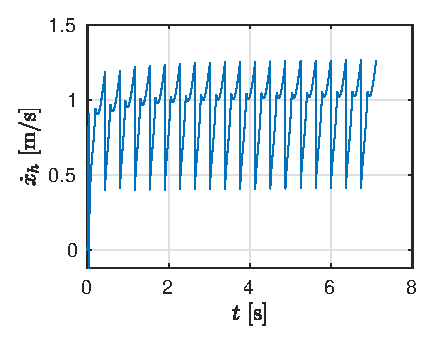
\includegraphics[width=\textwidth]{a04_dx_h}
			\caption{velocity of the hip}
		\end{center}
	\end{subfigure}
	\begin{subfigure}[h]{0.495\textwidth}
		\begin{center}
			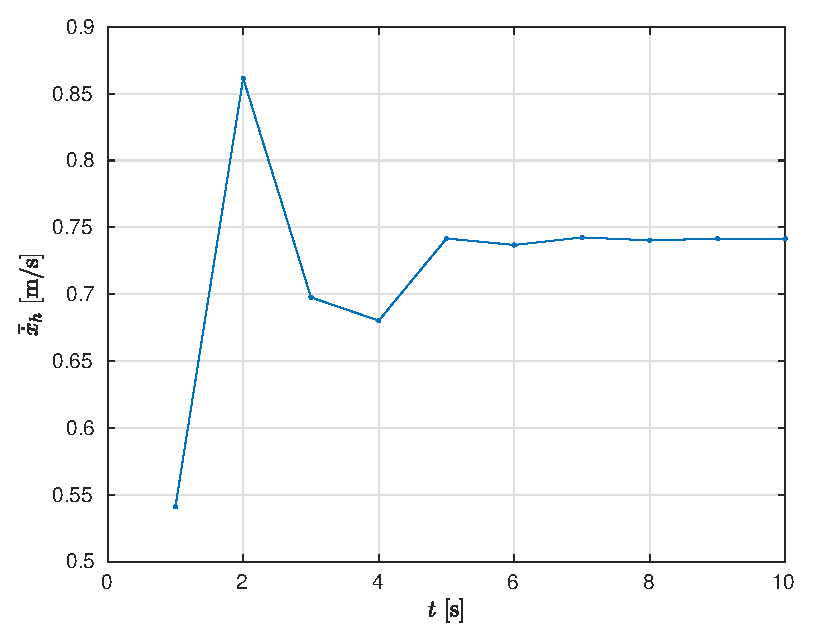
\includegraphics[width=\textwidth]{a04_average_dx_h}
			\caption{velocity of the hip averaged over the steps}
		\end{center}
	\end{subfigure}
	\caption{Velocity  of the hip in function of time / steps.}
\end{figure}

\begin{figure}[H]
	\begin{subfigure}[h]{0.495\textwidth}
		\begin{center}
			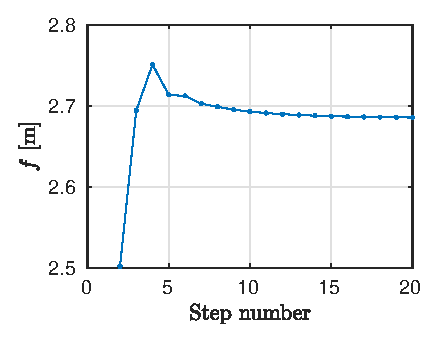
\includegraphics[width=\textwidth]{a04_step_frequency}
			\caption{step frequency}
		\end{center}
	\end{subfigure}
	\begin{subfigure}[h]{0.495\textwidth}
		\begin{center}
			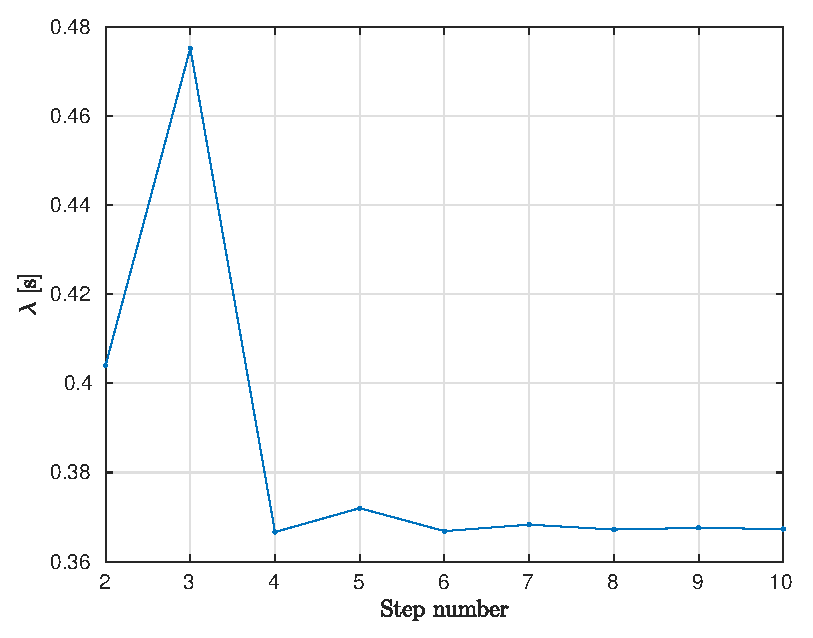
\includegraphics[width=\textwidth]{a04_step_lambda}
			\caption{step duration}
		\end{center}
	\end{subfigure}
	\caption{Regularity of the stepping.}
\end{figure}

%This gives us when computed a higher maximum and minimum velocity for the hip and swing foot. Furthermore, the input for $u_1$ and $u_2$ are also higher, while the angles for the three components of $q$ are smaller. This lead to a lower distance walked by the model over 9 steps, compared to the initial parameters. The nine steps are achieved faster but at the cost of smaller steps. The different metrics can be found here and are to be compared with those of the initial parameters when using the \verb|run\simulation.m| script.
%
%\begin{figure}[H]
%	\centering
%	\includegraphics[width=0.8\textwidth]{optimal/angle_velocity_vs_angle}
%	\caption{The angle velocity along the angle.}
%\end{figure}
%
%The maps appear to be more stable.
%
%\begin{figure}[H]
%	\centering
%	\includegraphics[width=0.8\textwidth]{optimal/angle_vs_time.png}
%	\caption{The angle of each component of $q$ throughout the simulation.}
%\end{figure}
%
%\begin{figure}[H]
%	\centering
%	\includegraphics[width=0.99\textwidth]{optimal/displacement_vs_step_number}
%	\caption{The displacement of the simulation over each steps.}
%\end{figure}
%
%\begin{figure}[H]
%	\centering
%	\includegraphics[width=0.99\textwidth]{optimal/speed_vs_time}
%	\caption{The angle velocity along the angle.}
%\end{figure}
%
%The maps appear to be more stable.
%
%\begin{figure}[H]
%	\centering
%	\includegraphics[width=0.99\textwidth]{optimal/torque_vs_time}
%	\caption{The controller input over time during the simulation}
%\end{figure}

\subsection{Reinforcment learning controller}

Because of problem of implementation, the RL controller was not completed, and thus didn't yield results.

\subsection{Virtual model controller}
